
\textbf{Off-policy distillation} trains the student on sequences generated by
another source, such as human-annotated data or outputs produced in advance by
a teacher model. Classical knowledge distillation is typically off-policy: the student learns to match
the teacher's output distribution on teacher-generated trajectories.
Informally, the student learns from model answers written by others.

\textbf{On-policy distillation} instead uses trajectories sampled online from
the student's current policy. The teacher provides token-level supervision on
these student-generated trajectories. After each student update, new
trajectories are sampled from the updated policy. In this setting, the student
produces its own answers, and the teacher evaluates how it should proceed.
 
This distinction is important because it affects \textbf{exposure bias}.
Under off-policy distillation, the student is trained primarily on high-quality
teacher or reference trajectories. During inference, however, it conditions
on its own outputs. An early mistake may move the student into a state rarely
represented in the training data, causing subsequent errors to accumulate.
Exposure bias thus arises partly from the mismatch between the
teacher/reference distribution observed during training and the
student-induced state distribution encountered during generation.

On-policy training reduces this mismatch by training on trajectories produced
by the current student policy. Even erroneous states encountered during
rollout become training examples, allowing the teacher to provide supervision
at states the student is likely to visit. This better aligns the training and
inference distributions, thereby mitigating exposure bias and compounding
errors.

On-policy training does not, however, eliminate exposure bias entirely.
Differences in teacher and student capabilities, low-quality rollouts,
distributional drift over long sequences, and optimization instability may
still create discrepancies between training and inference. More precisely,
on-policy distillation mitigates exposure bias at the data-distribution level
rather than removing it at its source. Its central advantage over purely
off-policy distillation is that the student learns not only what the teacher
would do along ideal trajectories, but also what the teacher recommends in
states reached by the student itself.

\begin{figure}[!ht]
    \centering
    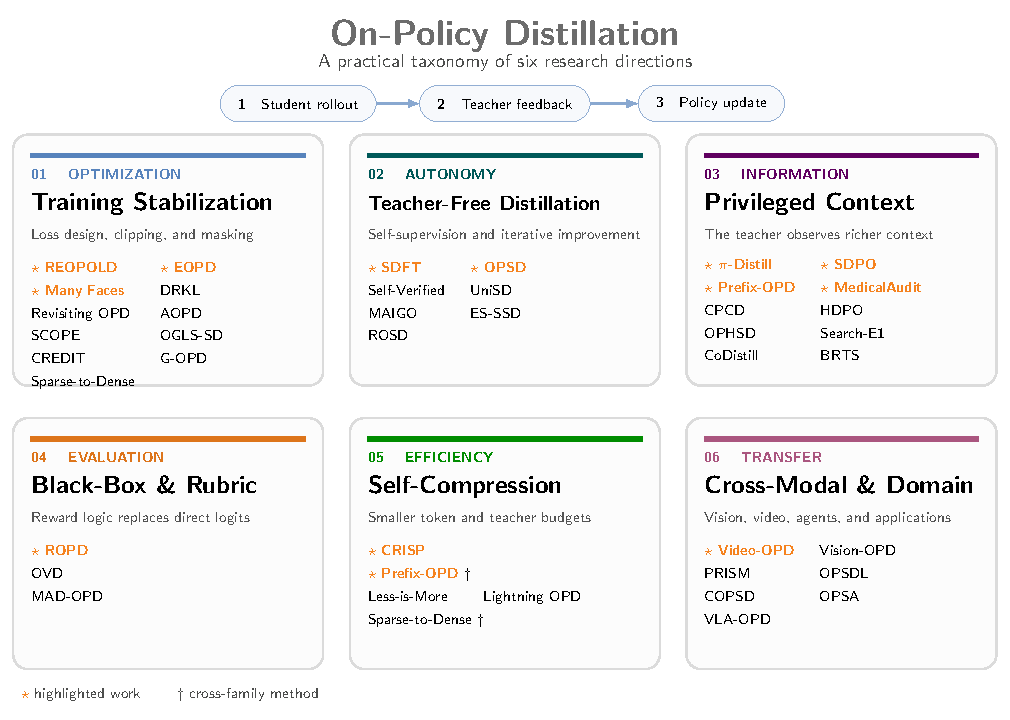
\includegraphics[width=\linewidth]{figures/opd_taxonomy.pdf}
    \caption{Six research directions in on-policy distillation, organized by the
    main source of innovation.}
    \label{fig:opd-taxonomy}
\end{figure}

\clearpage